\chapter{Introduction}
\label{ch:Introduction}

The purpose of this dissertation is to describe in detail
the methods used in extracting the $\beta$-decay asymmetry parameter
for the UCNA Experiment. This chapter hopes to motivate the inception
of the parameter of interest and its role in the theory of $\beta$-decay.
Also introduced are characteristics of the neutron itself with an
emphasis on ultracold neutrons (UCN), the namesake of the UCNA experiment.

%%%%%%%%%%%%%%%%%%%%%%%%%%%%%%%%%%%%%%%%%%%%%%%%%%%%%%%%%%%%%%%%%%%%%%%%%%%%%%%
%%%%%%%%%%%%%%%%%%%%%%%%%%%%%%%%%%%%%%%%%%%%%%%%%%%%%%%%%%%%%%%%%%%%%%%%%%%%%%%

\section{The Standard Model}
The Standard Model of particle physics encompasses everything we know about
interactions between particles and describes nature using the most fundamental
building blocks yet discovered. This section is used as an introduction
to these building blocks, the quarks and leptons, and to the mediators of the
interactions between them, to preface the upcoming descriptions of the neutron
and $\beta$-decay.

\subsection{The Building Blocks}

\subsection{The Forces}

\subsection{Symmetries}



%%%%%%%%%%%%%%%%%%%%%%%%%%%%%%%%%%%%%%%%%%%%%%%%%%%%%%%%%%%%%%%%%%%%%%%%%%%%%%%
%%%%%%%%%%%%%%%%%%%%%%%%%%%%%%%%%%%%%%%%%%%%%%%%%%%%%%%%%%%%%%%%%%%%%%%%%%%%%%%

\section{Properties of the neutron}
\label{sec:neutronProperties}
Let us take a moment to give a very brief introduction to the neutron to motivate the
upcoming sections. The majority of this dissertation can be read and mostly understood
without much knowledge of the theoretical description behind neutron $\beta$-decay,
so the properties of the neutron are a natural starting point.

The neutron is a net neutrally charged composite particle. The terms net and
composite hint at the inner structure of the neutron, made up of fundamental
particles called quarks, in this case two down ($d$) quarks and one up ($u$) quark.
The quarks carry charge, with the $u$ charge $+2/3$ and the $d$ charge
$-1/3$, so that the net charge of the neutron is zero. This can be compared
to the proton, another composite particle made up of three quarks (two $u$ and
one $d$ quark), whose net charge is $+1$ and the other nucleon found
within a nucleaus along with the neutron. Four other quarks exist,
the charm, strange, bottom, and top in order of increasing mass. The neutron
is the second lightest three-quark composite particle (baryon) 
behind only the proton.

\begin{figure}
  \centering
  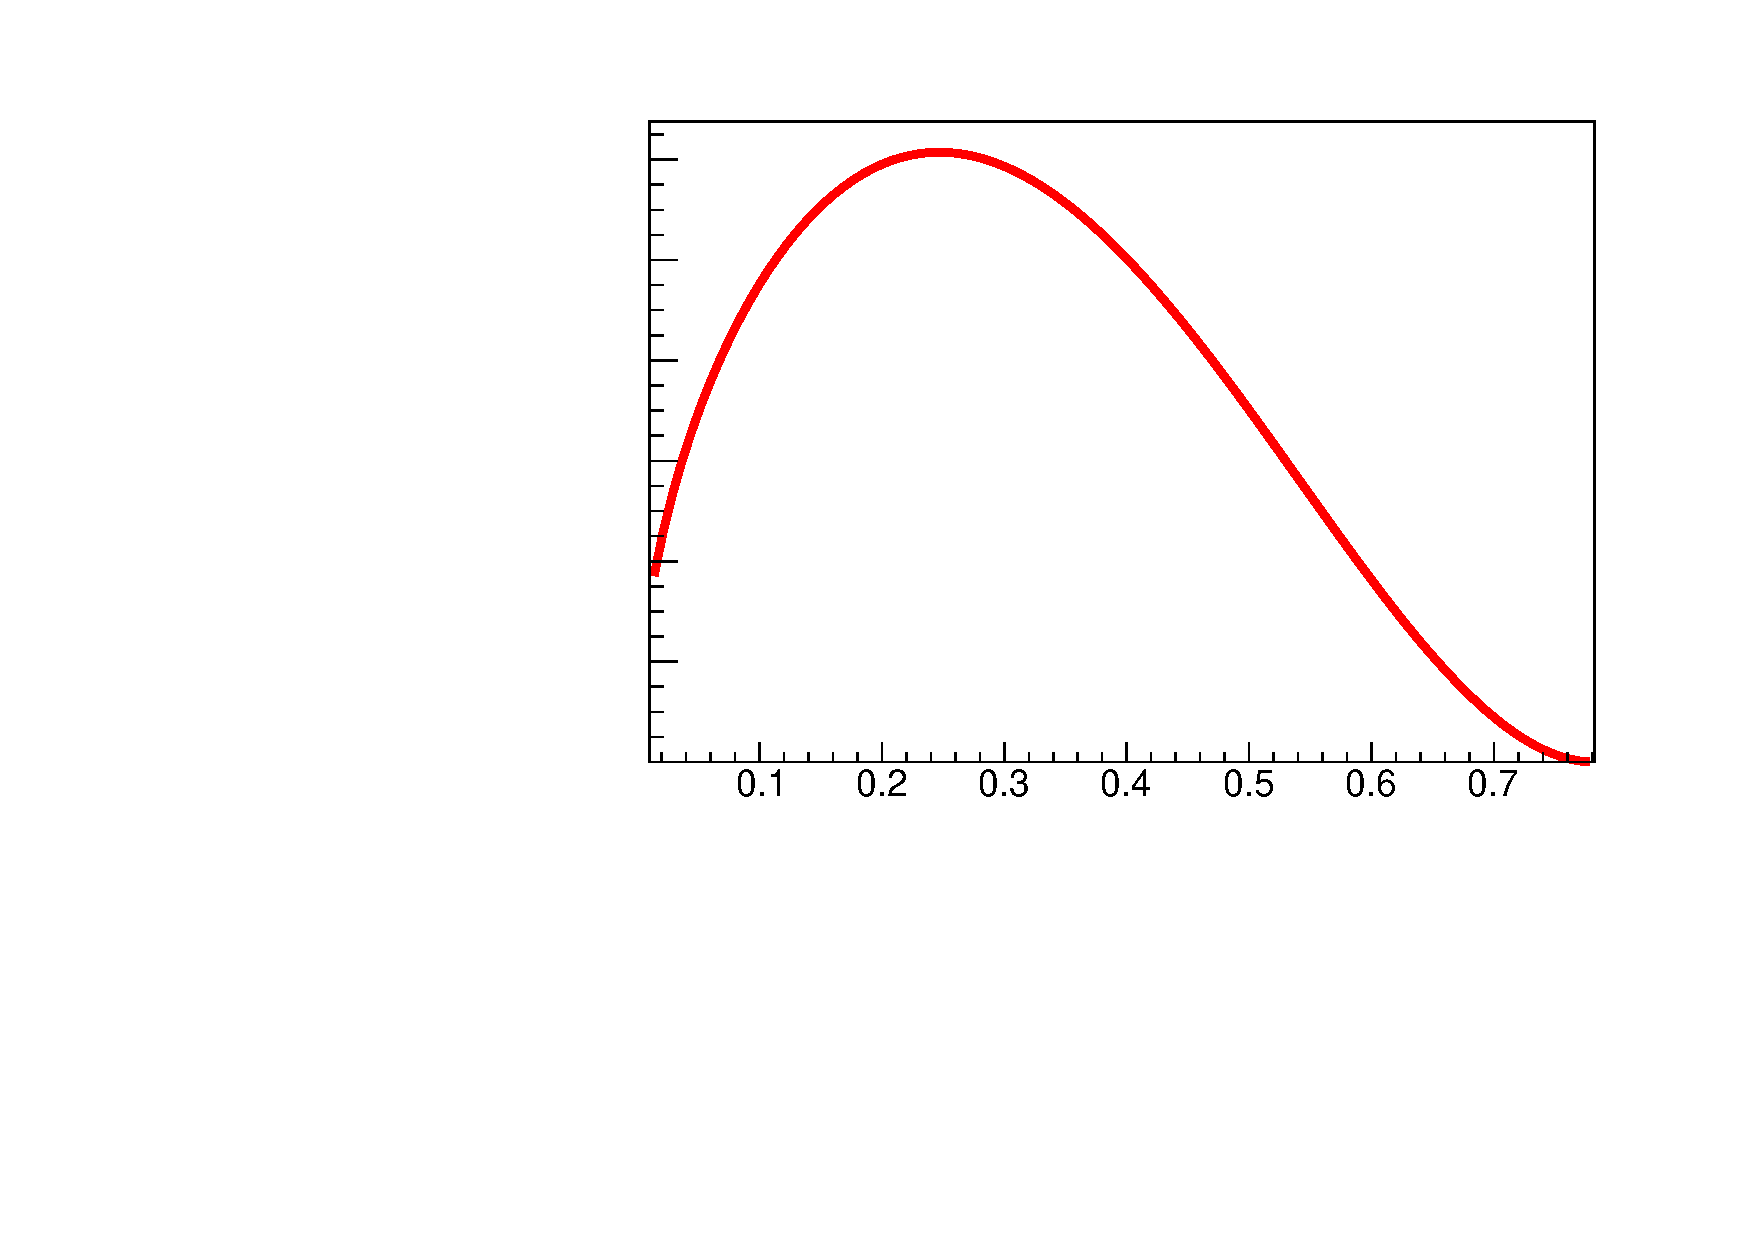
\includegraphics[page=1,scale=0.4]{1-Introduction/betaSpectrum.pdf}
    \caption{The electron kinetic energy spectrum in free neutron $\beta$-decay. The horizontal
      axis has units of energy in MeV in this case, but the shape of the spectrum
      is of general interest. Note that the decay probality does go to zero at zero
      MeV.}
  \label{fig:betaSpectrum}
\end{figure}

The free neutron undergoes $\beta$-decay, defined as a transition from the neutron
to a proton, electron, and electron anti-neutrino,
\begin{equation*}
  n\rightarrow p + e^- + \bar{\nu}_{e},
\end{equation*}
\noindent as is also seen in figure \ref{fig:pointInteraction}.
The three-body decay gives rise to a continuous energy spectrum
for the proton, electron, and anti-neutrino by conservation of energy and momentum.
The electron energy spectrum, the measurement of which is a primary focus of this
dissertation, is seen in figure \ref{fig:betaSpectrum}. The lifetime of the free neutron is
approximately fifteen minutes.


\section{$\beta$-decay and weak interactions: A brief history}

Prior to 1930, $\beta$-decay of nuclei was a polarizing topic of debate. Originally
only the decay electron was detected, and given such a two-body decay (the recoil
nucleus and the emitted electron being the two bodies) one would expect a discrete
electron energy defined by the difference in mass between mother and daughter
nuclei. Instead, a continuous energy spectrum was observed for the electron, which
initially led some to believe that energy conservation was moot. Others, like
Wolfgang Pauli, were not ready
to abandon energy conservation. He postulated that a neutral particle
could also be emitted in the decay. This third particle would share the energy available
in the reaction, explain the continuous energy distribution of the electron, and go
on undetected as it would not interact electromagnetically. The particle was termed
the neutrino by Fermi, and it would be a crux of Fermi's theory of $\beta$-decay.
A quarter century later, the existence of the neutrino would be confirmed
experimentally \cite{cowan1956detection}.

\subsection{Fermi's theory of $\beta$-decay}
After Pauli postulated the existence of the neutrino to explain the continuous energy
distribution of the $\beta$-decay electron, Fermi attempted to theoretically describe
the process in a similar manner to the theory of emission of
gamma radiation from an excited nucleus \cite{fermi1934,wilson1968fermi}.
His theory relied on two postulates: the existence of the neutrino and that the nucleus consisted
of heavy particles only, the neutron and the proton, both of which would turn out to be true.

\begin{table}[h]
  \caption{Transformation behavior of all possible bilinear covariants.} 
  \centering
  \begin{tabular}{l c }
    \hline \hline \\ [-1.75ex]
    $\bar{\psi}\psi$ & scalar \\ [0.50ex]
    $\bar{\psi}\gamma^5\psi$ & pseudoscalar \\ [0.50ex]
    $\bar{\psi}\gamma^{\mu}\psi$ & vector \\ [0.50ex]
    $\bar{\psi}\gamma^{\mu}\gamma^5\psi$ & axial vector \\ [0.50ex]
    $\bar{\psi}\sigma^{\mu\nu}\psi$ & antisymmetric tensor \\ [0.50ex]   
    \hline
  \end{tabular}
  \label{tab:bilinearCov}
\end{table}

Fermi's interaction Hamiltonian took the form (written in a different manner from Fermi's original
paper on the subject for the sake of clarity) 
%
\begin{equation}
  H = C_V\big( \bar{\psi}_p \gamma_\mu \psi_n \big) \big( \bar{\psi}_e \gamma^\mu \psi_\nu \big), 
\end{equation}
%
where $\bar{\psi} \gamma_\mu \psi$ is a vector current (see table \ref{tab:bilinearCov}). The assumption
that the current-current interaction would be of the vector-vector variety was a natural
choice as this is the case for electromagnetism.

\begin{figure}
  \centering
  \centering
  %\begin{tabular} {cc}
  \subfloat[Contact Interaction at the particle level]{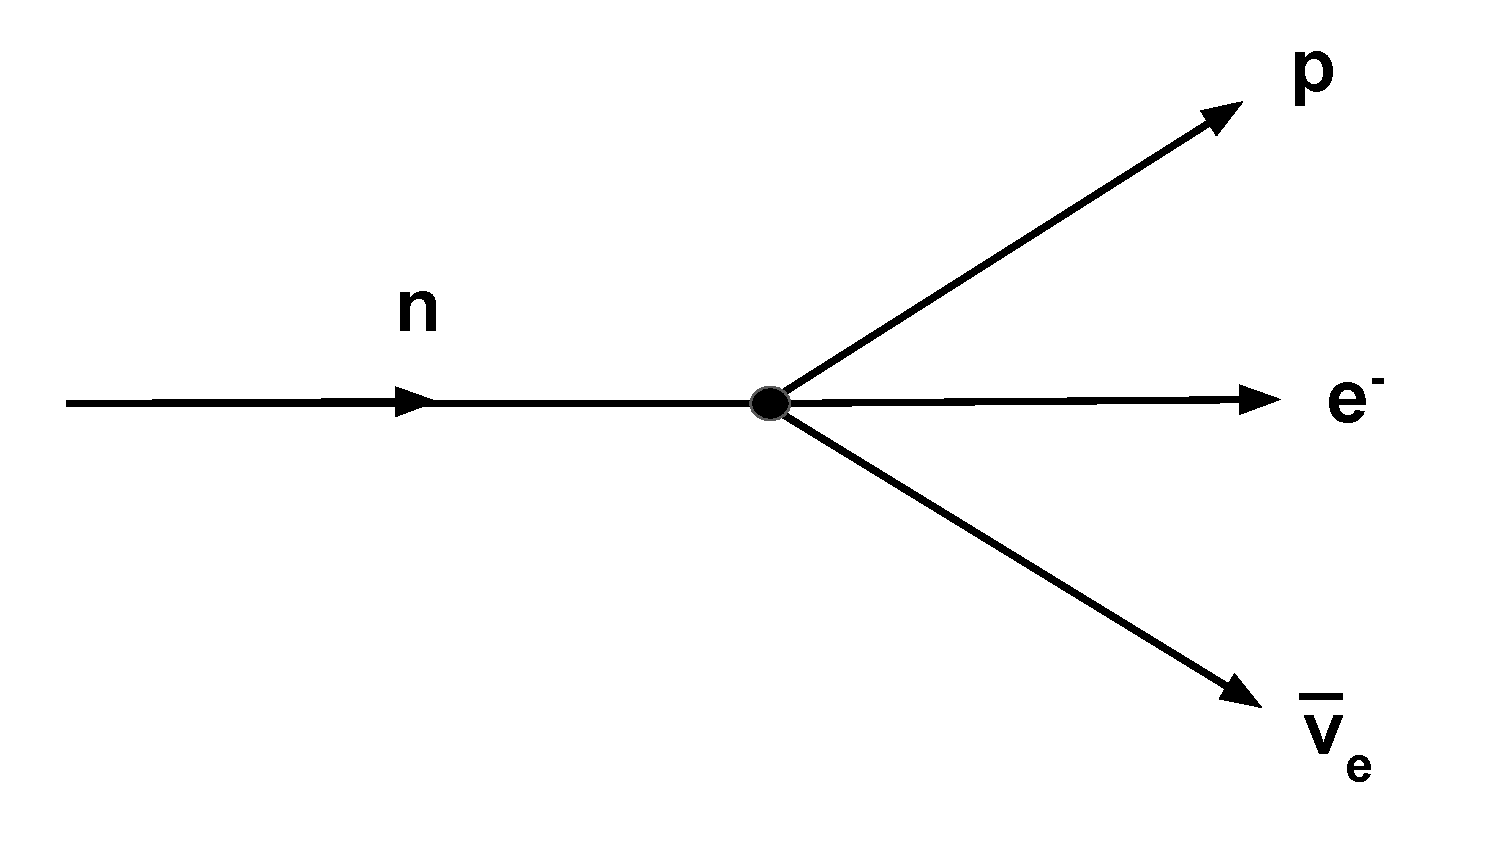
\includegraphics[page=1,scale=0.4]{1-Introduction/pointInteraction.pdf}}\\
  \subfloat[Quark level decay]{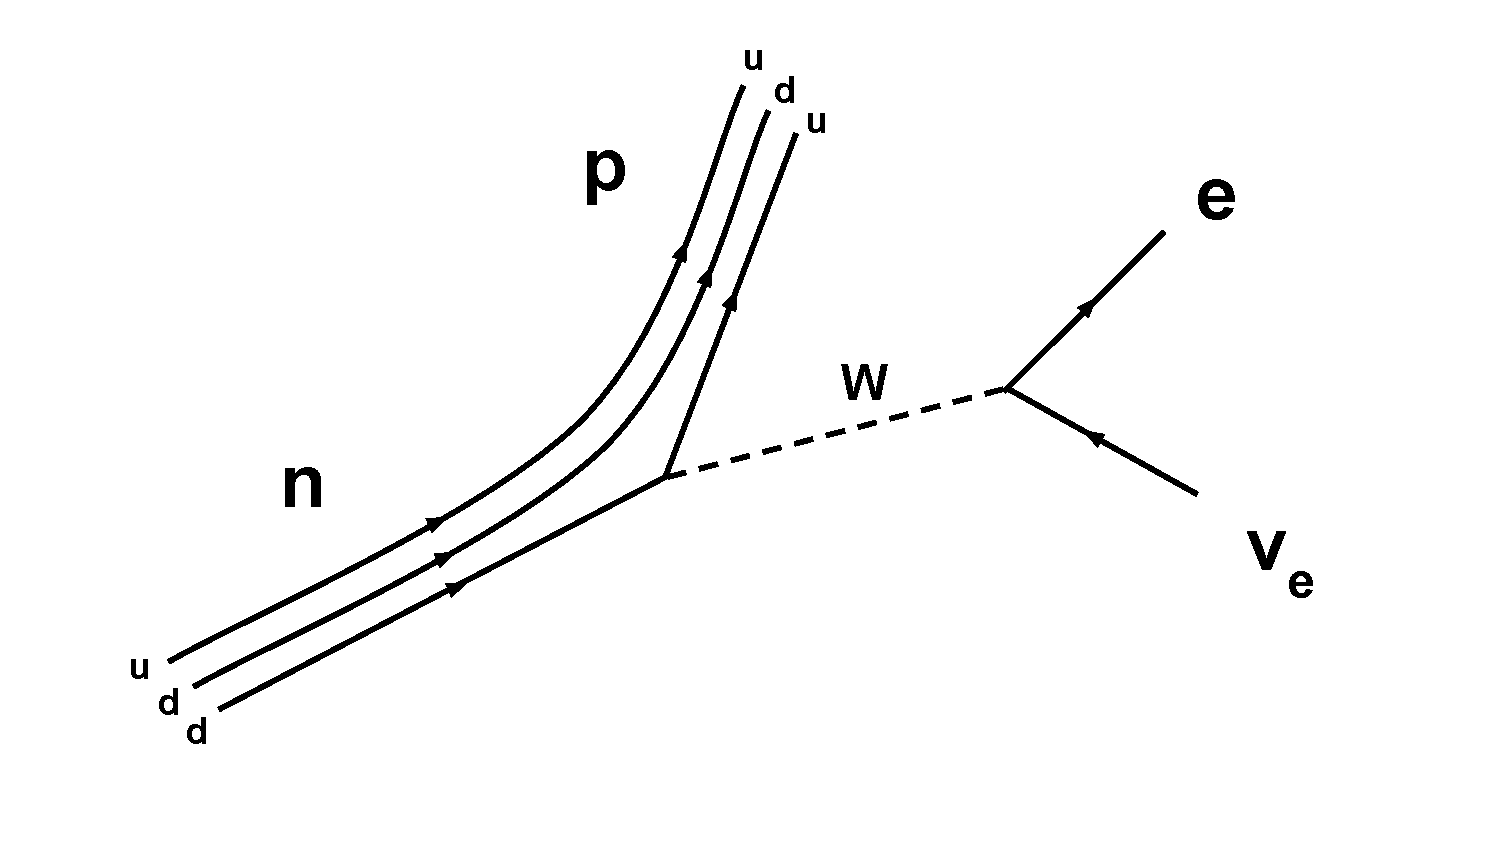
\includegraphics[page=1,scale=0.4]{1-Introduction/quarkInteraction.pdf}}
  %\end{tabular}
  \caption{The contact interaction of Fermi's theory of $\beta$-decay is shown in a.). The theory is
    capable of describing other processes which move one of the outgoing particle lines
    to the left side, like electron capture by the proton producing a neutron and an
    electron neutrino. b.) shows the decay at the quark level, where the initial state is the
    quark makeup of the neutron, and the subsequent decay of one of the down quarks into an up
    quark creates the W boson which decays into the electron and electron anti-neutrino.}
  \label{fig:pointInteraction}
\end{figure}

Fermi's theory of $\beta$-decay treats the decay as a four-point contact interaction
(see figure \ref{fig:pointInteraction}), where
the currents are evaluated at the same point in space and time \cite{renton1990}. For those
familiar with quantum field theory within the Standard Model, this differs from the typical
interaction Hamiltonian as there is no propagator, or force carrier, to mediate the
interaction between the two currents. The small momentum transfer in nuclear
$\beta$-decay compared to the mass of the $W$ bosons makes this point interaction a good
approximation at low energies.  The theory
worked well at predicting the energy spectrum of the electron from which
Fermi deduced that the neutrino must be nearly massless, but suffered one flaw. The vector
nature of the theory did not permit the observed allowed nuclear $\beta$-decay transitions
which can transform the spin of the decaying nucleus. This was pointed out by Gamow and Teller in
1936 \cite{gamow1936}, where they show that a current-current interaction that transforms like
a pseudovector properly assigns the spins of the products in thorium decays. As such,
one can generalize Fermi's theory by including all possible bilinear covariant terms that
satisfy Lorentz invariance:
%
\begin{multline}
  H = C_S\big( \bar{\psi}_p \psi_n \big) \big( \bar{\psi}_e  \psi_\nu \big) 
  +C_V\big( \bar{\psi}_p \gamma_\mu \psi_n \big) \big( \bar{\psi}_e \gamma^\mu \psi_\nu \big) \\
  +C_T\big( \bar{\psi}_p \sigma^{\mu\nu} \psi_n \big) \big( \bar{\psi}_e \sigma^{\mu\nu} \psi_\nu \big) 
  +C_A\big( \bar{\psi}_p \gamma_\mu \gamma^5 \psi_n \big) \big( \bar{\psi}_e \gamma^\mu \gamma^5 \psi_\nu \big) 
  +C_P\big( \bar{\psi}_p  \gamma^5 \psi_n \big) \big( \bar{\psi}_e  \gamma^5 \psi_\nu \big),
  \label{eq:FermiFull}
\end{multline}
%
where the coefficients quantify the coupling to each respective current.

\subsubsection{Fermi and Gamow-Teller Transitions}

This shortcoming of Fermi's original vector-vector interaction
lends itself to the definition of
two types of allowed $\beta$-decay transitions. The Fermi transition proceeds through the
scalar and vector currents with $\Delta J=0$ and no parity change. Gamow-Teller transitions
correspond to the axial vector and tensor currents and have $\Delta J=0,\pm1$ with no parity change,
but excluding the $0^+\rightarrow 0^+$ nuclear transitions. The pseudoscalar terms does not
contribute to the amplitude in the low energy limit \cite{renton1990}.
 

\subsection{Parity Violation in Weak Decays}

\subsubsection{Lee and Yang}

Prior to the 1950's, all discrete symmetries (parity, charge conjugation, and time reversal)
were thought to be conserved separately for all interactions in nature. A dilemma arose when
two particles, called the $\tau$ and $\theta$ mesons at the time, posessed the same mass
and charge as the $K^+$ meson, but decayed to different final states of parity. The $\tau$ decayed into three pions
and the $\theta$ into two pions. The initial classification of the two observably identical particles into
two different particles was logical given that parity conservation was then sacrosanct,
but in 1956 Lee and Yang proposed a very different solution to the problem. They realized that
there was no evidence that parity must be conserved in the weak interaction.
In the full expression of Fermi's theory (equation \ref{eq:FermiFull}),
while including all possible combinations of bilinear covariants, there was no mixing between the
individual currents and each individual current-current term transforms like a scalar. For example,
two individual axial vector currents would each transform as
$P(\bar{\psi}_p \gamma_\mu \gamma^5 \psi_n) \rightarrow -\bar{\psi}_p \gamma_\mu \gamma^5 \psi_n$ under parity, but the
muliplication of two such terms transforms like a scalar. Thus, none of the terms in \ref{eq:FermiFull})
are capable of violating parity, as the Hamiltonian would remain invariant under a parity transformation. 

In their 1956 paper \cite{leeyang1956}, Lee and Yang modified the weak ineraction Hamiltonian
by including the possibility of a pseudoscalar current-current interaction, namely
%
\begin{multline}
  H = \bar{\psi}_p \psi_n \big( C_S\bar{\psi}_e  \psi_\nu + C'_S\bar{\psi}_e \gamma^5 \psi_\nu \big) \\
  + \bar{\psi}_p \gamma_\mu \psi_n  \big( C_V\bar{\psi}_e \gamma^\mu \psi_\nu + C'_V\bar{\psi}_e \gamma^\mu \gamma^5 \psi_\nu \big) 
  + \bar{\psi}_p \sigma^{\mu\nu} \psi_n \big( C_T\bar{\psi}_e \sigma^{\mu\nu} \psi_\nu + C'_T\bar{\psi}_e \sigma^{\mu\nu} \gamma^5 \psi_\nu \big)\\
  + \bar{\psi}_p \gamma_\mu \gamma^5 \psi_n \big( C_A\bar{\psi}_e \gamma^\mu \gamma^5 \psi_\nu + C'_A\bar{\psi}_e \gamma^\mu \psi_\nu \big) 
  + \bar{\psi}_p  \gamma^5 \psi_n \big( C_P\bar{\psi}_e  \gamma^5 \psi_\nu + C'_P\bar{\psi}_e \psi_\nu \big).
  \label{eq:leeyang}
\end{multline}
%
If any of the $C'_i$ coefficents are nonzero, parity would not be conserved due to
the scalar-pseudoscalar form of the current-current interactions that are labelled by
the primed coefficients.

Along with the inclusion of potential parity violating terms in the Hamiltonian, Lee and Yang
presented several potential tests of parity violation in the weak sector. One such proposition
was the measurement of the correlation between the spin of a polarized nucleus and
the momentum of the $\beta$-decay electron.

\subsubsection{Discovery of Parity Violation}

Following the publication of Lee and Yang's newly modified theory of $\beta$-decay, C. S. Wu
and collaborators designed an experiment to test the potential violation
of parity in the $\beta$-decay of $^{60}\mathrm{Co}$
($^{60}\mathrm{Co} \rightarrow {^{60}\mathrm{Ni}} + e^- + \bar{\nu}_e$) \cite{wu1957}. The premise of the experiment
was simple: place an electron detector along the $+z$ axis, polarize the $^{60}\mathrm{Co}$ nuclei
using a magnetic field in the $\pm z$ direction, and measure the electron rate in each polarization
configuration. If parity is violated, a clear asymmetry would be present between the two polarizations,
which is precisely what was discovered and can be seen in figure \ref{fig:wuData}.

\begin{figure}[h]
  \centering
  \includegraphics[scale=0.50]{1-Introduction/wuData.png}  
  \caption{Data from C. S. Wu's experiment measuring the correlation between the emitted
    direction of the electron from the decay of polarized $^{60}\mathrm{Co}$. The two
    curves represent the counting rates when the nuclei were oriented in opposite
    directions with respect to the electron detector. The existence of a splitting
    indicatesa violation of parity as the electrons are preferentially emitted in the
    direction opposite the spin.}
  \label{fig:wuData}
\end{figure}

The measurement showed that the electrons were preferentially
emitted in the direction opposite the spin of the nuclei, which indicates parity violation due to
the position inverted scenario not being observable. This is evident when considering that
a correlation between the the spin and the momentum takes the form $\boldsymbol{\sigma \cdot p}$.
The spin is a type of angular momentum and transforms as an axial vector under spatial inversion
($P\boldsymbol{\sigma}=\boldsymbol{\sigma}$), while the momentum is a normal vector and
simply changes sign under parity ($P\boldsymbol{p}=-\boldsymbol{p}$). Thus the existence of
such a term in the decay rate (as will be shown in section \ref{ssec:correlations}) makes the
decay rate noninvariant under a parity transformation, and the position inverted scenario
is automatically impossible since the spin vector would not change but we would expect to see
the electron direction flip. This would result in electrons emitted aligned with the direction
of the spin, which is not the observed case. As indicated by Wu,
the fact that the electrons prefer emission in the direction opposite
to the spin indicates that the $C'_i=-C_i$ for whichever
interaction current was responsible for the symmetry breaking. From the theory presented thus far,
the interaction involved was either axial vector or tensor, because decay of
$^{60}\mathrm{Co} (J^p=5^+) \rightarrow {^{60}\mathrm{Ni}}(J^p=4^+)$ proceeds stricly through
the Gamow-Teller transition. Whether the tensor or axial vector current (or both) was responsible
was yet to be determined.

It should be noted that, following the news of Wu's result, Garwin, Lederman, and
Weinrich \cite{garwin1957} from Columbia confirmed
that parity is violated using the subsequent decays of $\pi^+ \rightarrow \mu^++\nu_\mu$
followed by $\mu^+ \rightarrow e^+ + \bar{\nu}_e + \nu_\mu$. This was another process
recommended by Lee and Yang. The premise is that the chiral odd neutrino in the first decay
forces the muon to be polarized in the direction of its momentum to conserve angular
momentum. The polarized muon then decays and can thus be analyzed much like one would analyze the
$\beta$-decay of a polarized nucleus, looking for correlations between the polarization and
the decay electron. The results were again conclusive that parity is not conserved in the weak
interaction.

\subsection{Correlation Coefficients} \label{ssec:correlations}
Taking the interaction Hamiltonian from Lee and Yang with all generalized terms included,
Jackson, Treiman, and Wyld \cite{jackson1957a,jackson1957b} first derived an expression
for the differential decay rate for polarized nuclei as a function of the emitted electron momentum
and spin, the neutrino momentum, and the nuclear spin of the decaying nucleus.
Ebel and Feldman \cite{ebel1957} added terms to the expression of Jackson, Treiman, and Wyld,
and, under the assumption that the spin of the mother nucleus and the spin of the outgoing electron
are observable, this gives
%
\begin{multline}
  \frac{d\Gamma}{dE_e dE_\nu d\Omega_e d\Omega_\nu} = \frac{1}{2} \frac{F(\pm Z, E_e)}{\big( 2\pi \big)^5}
  p_e E_e \big( E^0 - E_e \big)^2 \\ \times \xi 
  \Bigg\{ 1 + a\frac{\boldsymbol{p_e \cdot p_\nu}}{E_e E_\nu} + b\frac{m_e}{E_e} 
  + \frac{\boldsymbol{\langle J \rangle}}{J} \boldsymbol{\cdot} \Bigg[ A\frac{\boldsymbol{p_e}}{E_e}
    + B\frac{\boldsymbol{p_\nu}}{E_\nu} + D\frac{\boldsymbol{p_e \times p_\nu}}{E_e E_\nu}\Bigg] \\
  + \Bigg[ \frac{J(J+1)-3\langle (\boldsymbol{J \cdot \hat{\jmath}})^2 \rangle}{J(2J-1)} \Bigg]
  \Bigg( c\Bigg[ \frac{\boldsymbol{p_e} \times \boldsymbol{p_\nu}}{3E_eE_\nu} -
    \frac{(\boldsymbol{p_e\cdot \hat{\jmath}})(\boldsymbol{p_\nu\cdot \hat{\jmath}}) }{E_eE_\nu} \Bigg]
  + I \Bigg[ \frac{1}{3}\frac{\boldsymbol{\sigma \cdot p_\nu}}{E_\nu}
    - \frac{(\boldsymbol{\sigma \cdot \hat{\jmath}})(\boldsymbol{p_\nu \cdot \hat{\jmath}})}{E_\nu} \Bigg] \\
  + K'\frac{\boldsymbol{\sigma \cdot p_e}}{E_e+m_e} \Bigg[ \frac{1}{3}\frac{\boldsymbol{p_e \cdot p_\nu}}{E_e E_\nu}
    - \frac{(\boldsymbol{p_e \cdot \hat{\jmath}})(\boldsymbol{p_\nu \cdot \hat{\jmath}})}{E_e E_\nu} \Bigg] 
  + M \Bigg[ \frac{1}{3}\frac{\boldsymbol{\sigma \cdot p_e \times p_\nu}}{E_e E_\nu}
    - \frac{(\boldsymbol{\sigma \cdot \hat{\jmath}})(\boldsymbol{\hat{\jmath} \cdot p_e \times p_\nu })}{E_e E_\nu} \Bigg] \Bigg) \\
  + \boldsymbol{\sigma} \cdot \Bigg[ N\frac{\langle \boldsymbol{J} \rangle}{J}
    + Q\frac{\boldsymbol{p_e}}{E_e+m_e}\Bigg(\frac{\langle \boldsymbol{J} \rangle}{J}\boldsymbol{\cdot} \frac{\boldsymbol{p_e}}{E_e}\Bigg)
    + R\frac{\langle \boldsymbol{J} \rangle}{J}\boldsymbol{\times} \frac{\boldsymbol{p_e}}{E_e}
    + S\frac{\langle \boldsymbol{J} \rangle}{J} \frac{\boldsymbol{p_e\cdot p_\nu}}{E_e E_\nu} \\
    + T\frac{\boldsymbol{p_e}}{E_e}\frac{\langle \boldsymbol{J} \rangle}{J} \boldsymbol{\cdot} \frac{\boldsymbol{p_\nu}}{E_\nu}
    + U\frac{\boldsymbol{p_\nu}}{E_\nu}\frac{\langle \boldsymbol{J} \rangle}{J} \boldsymbol{\cdot} \frac{\boldsymbol{p_e}}{E_e}
    + W\frac{\boldsymbol{p_e}}{E_e+m_e}\frac{\langle \boldsymbol{J} \rangle}{J} \boldsymbol{\cdot} \frac{\boldsymbol{p_e \times p_\nu}}{E_e E_\nu}
    \Bigg]
  + V\frac{\langle \boldsymbol{J} \rangle}{J} \boldsymbol{\cdot} \frac{\boldsymbol{\sigma \times p_\nu}}{E_\nu}
  \Bigg\}
  \label{eq:jackson}
\end{multline}
%
where $F(\pm Z, E_e)$ is the Fermi function (a shape correction to the spectrum
from coulomb interactions), $E$ is the energy of a given particle, $E^0$ is the endpoint
energy of the electron, $\boldsymbol{p}$ is the particle momentum, $\boldsymbol{J}$ is the spin of the
decaying nucleus (or nucleon), and $\sigma$ is the spin of the electron. All of the correlation coefficients
are functions of the coupling constants in the weak Hamiltonian (see equation \ref{eq:leeyang}),
as is $\xi$. The correlation coefficients and $\xi$ are also functions of Fermi and Gamow-Teller
transition amplitudes \footnote{For the complete defitions see \cite{jackson1957a,jackson1957b,ebel1957}}.

Foreshadowing upcoming sections, we write down the definitions of $\xi$ and $A\xi$ (ignoring Coulomb
corrections):
%
\begin{equation}
  \xi = |M_F|^2\big(|C_S|^2+|C_V|^2+|C'_S|^2+|C'_V|^2\big)+|M_{GT}|^2\big(|C_T|^2+|C_A|^2+|C'_T|^2+|C'_A|^2\big)
\end{equation}
%
\begin{multline}
  A\xi = 2\mathrm{Re}\bigg[\pm |M_{GT}|^2 \lambda_{J'J}\big(C_TC'^*_T-C_AC'^*_A \big) \\
    + \delta_{J'J}|M_F||M_{GT}|\bigg( \frac{J}{J+1} \bigg)^{\frac{1}{2}}\big(C_SC'^*_T+C'_SC^*_T -C_VC'^*_A-C'_VC^*_A \big) \bigg]
\end{multline}
where
\begin{equation}
\lambda_{J'J} =
\begin{dcases}
  1, & J\rightarrow J'=J-1 \\
  \frac{1}{J+1}, &  J\rightarrow J'=J \\
  \frac{-J}{J+1}, &  J\rightarrow J'=J+1 \\
\end{dcases}
\end{equation}
The rest of the coefficients have varying combinations of the the complex coupling
constants $C$, $C'$, and the Fermi and
Gamow-Teller amplitudes.

Jackson, Treiman, and Wyld concisely state the impact these terms have on tests of C, P, and
T invariance:
\begin{displayquote}
Invariance with respect to space inversion implies that the coupling constants $C'$
vanish (or alternatively the $C$ vanish). Invariance with respect to charge
conjugation implies that the constants $C$ are real and the constants $C'$
pure imaginary, up to an overall phase. Invariance under time reversal
would imply that all coupling constants $C$, $C'$ are real, again up to an
overall phase.
\end{displayquote}

Measurements of the correlation parameters in nuclear systems shed light on the
relationships between the different coupling constants, but it would take observations
of the behavior of the observed neutrinos and electrons to determine the true structure
of the interaction Hamiltonian.

\subsection{$V-A$ Structure}

By 1956, the theory of the weak interaction had developed from a purely vector current-current
process into
a combination of all possible Lorentz invariant current-current interactions and finally to the potential mixture
of current-current terms that transform as scalars and pseudoscalars in order to accomodate
parity violation. At this point, the theory needed to rely on experiment to determine
which couplings were nonzero.

In early 1957, upon Wu reporting preliminary results regarding the large asymmetry seen in the $\beta$-decay
of $^{60}\mathrm{Co}$ to Lee and Yang, the duo developed a two component theory
of the neutrino where a massless neutrino exists in a predefined polarization, or that
its spin is always oriented in the same direction with respect to its momentum \cite{lee1957}
\footnote{Technically this only applies to neutrinos that interact via
  the weak interaction, but seeing as neutrinos are only
  observed to interact weakly, this can be generalized to all observable neutrinos. Also, Lee and
  Yang's theory had the wrong sign for the $\boldsymbol{\sigma \cdot p}$ of the neutrino.}.
This was the first theory to indicate that the weak interaction coupled only to particles
of a certain handedness, where right (left) handedness refers to eigenstates with eigenvalues of the
chirality projection operator ($P_{\pm} = (1\pm \gamma^5)/2$) equal to $+1\mathrm{ }(-1)$. This operator
should look familiar, as it is the term Lee and Yang inserted into Fermi's theory of $\beta$-decay
when $C_i=C'_i$. 

In 1958, Feynman and Gell-Mann \cite{feynman1958} (and separately Sudarshan and Marshak
\cite{sudarshan1958}) would report the currently accepted V-A (vector minus axial vector)
theory of the weak interaction. The name derives from the form of the two currents in the
current-current Hamiltonian.
The new theory involved the coupling of the weak current to strictly left-handed particles and right-handed
antiparticles. More simply, a massless neutrino will always have helicity
$\boldsymbol{\sigma \cdot p}/p = -1$ while an anti-neutrino will have $\boldsymbol{\sigma \cdot p}/p = +1$,
where the fact that helicity and chirality are one in the same for massless particles is utilized.
The form of the V-A interaction Hamiltonian
%
\begin{equation}
  H = G_F \Big(\bar{\psi}_n \gamma_\mu(1-\gamma^5)\psi_p \Big)\Big(\bar{\psi}_{\bar{\nu}} \gamma^\mu(1-\gamma^5)\psi_e \Big),
  \label{eq:VminusA}
\end{equation}
%
where $G_F$ is the Fermi coupling constant of the weak interaction,
assumes that the V-A structure is universal within the weak interaction\footnote{This is
  only strictly true for the charged weak interaction (so a change in charge occurs in each current),
  but at this time only the charged weak interaction
  was known.}.

The theories of Feynman and Gell-Mann (and Sudarshan and Marshak)
explained the observations at that time
regarding the weak interaction. Then, also in 1958, confirmation of the V-A theory arrived when
Goldhaber, Gradzins, and Sunyar indirectly measured
the helicity of the neutrino in electron capture on $^{152}\mathrm{Eu}$ and determined the
emitted neutrino was indeed left-handed
\cite{goldhaber1958,greiner1996}. It should be noted that these two theories differed from that of
Lee and Yang in the definition of the chirality of the particles ($-$) and anti-particles ($+$), where
Lee and Yang had the opposite definition.

Now one may be tempted to ask why only the vector and axial vector components of the original
parity violating Hamiltonian remain, and this is easily answered by imagining that the
left-handed coupling was discovered prior to modification of the Hamiltonian in equation
\ref{eq:FermiFull} by Lee and Yang to account for parity violation. We can define the left-handed
particle states as (up to a factor of $1/2$ left off for convenience)
%
\begin{equation}
  \psi_L = (1-\gamma^5)\psi.
\end{equation}
%
Then using this in the current yields
%
\begin{equation}
  \bar{\psi}_{1,L} O_i \psi_{2,L} = \overline{(1-\gamma^5)\psi_{1}} O_i (1-\gamma^5)\psi_{2}
\end{equation}
%
where $O_i$ refers to all of the operators which produce S, V, T, A, and P bilinear covariants
from table \ref{tab:bilinearCov} and subscript 1,2 refers to two different particle states.
The $O_i$ are those that are present in \ref{eq:FermiFull}.

\begin{table}[h]
  \caption{The chirality projected operators.} 
  \centering
  \begin{tabular}{c c c }
    \hline \hline \\ [-1.75ex]
    Type & $O_i$ & $O'_i$ \\ [0.50ex]
    \hline \\ 
    S & $1$ & 0 \\ [0.50ex]
    P & $\gamma^5$ & 0 \\ [0.50ex]
    V & $\gamma^{\mu}$ & $\gamma^\mu(1-\gamma^5)$ \\ [0.50ex]
    A & $\gamma^{\mu}\gamma^5$ & $-\gamma^\mu(1-\gamma^5)$ \\ [0.50ex]
    T & $\sigma^{\mu\nu}$ & 0 \\ [0.50ex]   
    \hline
  \end{tabular}
  \label{tab:operatorPrime}
\end{table}

Now it can be shown that
%
\begin{align*}
  \bar{\psi}_{1,L} O_i \psi_{2,L} &= \overline{(1-\gamma^5)\psi}_{1} O_i (1-\gamma^5)\psi_{2} \\
  &= \Big((1-\gamma^5)\psi_{1}\Big)^\dagger \gamma^0 O_i (1-\gamma^5)\psi_{2} \\
  &= \psi^\dagger_{1}(1-\gamma^5)^\dagger \gamma^0 O_i (1-\gamma^5)\psi_{2} \\
  &= \psi^\dagger_{1}(1-\gamma^5) \gamma^0 O_i (1-\gamma^5)\psi_{2} \\
  &= \psi^\dagger_{1}\gamma^0(1+\gamma^5) O_i (1-\gamma^5)\psi_{2} \\
  &= \bar{\psi_{1}}(1+\gamma^5) O_i (1-\gamma^5)\psi_{2} 
\end{align*}
%
where the relations ${\gamma^5}^\dagger = \gamma^5$ and $\{\gamma^5,\gamma^i\}=0$ were used.

Then, if we define
\begin{equation*}
  O'_i = (1+\gamma^5) O_i (1-\gamma^5),
\end{equation*}
we can calculate how all of the S, V, T, A, and P operators transform. This is shown in table
\ref{tab:operatorPrime}, where we see that only the vector and axial vector terms remain, and they
appear with the same $\gamma^\mu(1-\gamma^5)$ factor up to a sign! Thus, these are the only
currents which can contribute in the interaction Hamiltonian \cite{greiner1996}.



%Several experimental efforts (cite experiments) at the time indicated that the emitted particles
%(antiparticles) from weak decay processes were in helicity states of $-1$ ($+1$), where helicity
%is defined as $\Lambda = \boldsymbol{\sigma \cdot p}/p$ and the spin and momentum are both of the emitted
%particle. This means that in $\beta^-$-decay, the emitted electron has negative helicity and the
%antineutrino has positive helicity. This may lead one to believe that the weak force couples only
%to negative (positive) helicity eigenstates for particles (antiparticles), and as such the
%Hamiltonian would include the helicity projection operator $P_{\pm} = (1\pm \Lambda)/2$ to select
%only the proper helicity states from the wavefunction. This has one major issue: the helicity
%operator is not Lorentz invariant for massive particles. Thus a Lorentz boost to a
%reference frame moving in the direction of particle motion but with speed greater than that of
%the particle 

\subsection{Renormalizing the Hadronic Current}

The forms of both the hadronic current ($\bar{\psi}_p \gamma_\mu(1-\gamma^5)\psi_n$) and
leptonic current ($\bar{\psi}_\nu \gamma_e(1-\gamma^5)\psi_{\bar{\nu}}$) in \ref{eq:VminusA} indicate
that the vector and axial vector currents possess the same coupling constants, or that
they contribute equally in the weak interaction. For the leptonic current this is the case
as the particles participating are true point particles (and the equal relative strengths are
what is meant by parity is violated maximally in the weak interaction), but what about the
hadronic current? To account for potential differences in the hadronic current, the
Hamiltonian is modified slightly,
%
\begin{equation}
  H = G_F \Big(\bar{\psi}_p \gamma_\mu(g_V-g_A\gamma^5)\psi_n \Big)\Big(\bar{\psi}_{e} \gamma^\mu(1-\gamma^5)\psi_{\bar{\nu}} \Big),
  \label{eq:VminusA2}
\end{equation}
%
which lends itself to the definition
%
\begin{equation}
  \lambda \equiv \frac{g_A}{g_V}.
\end{equation}

Within the nucleon, there exists a sea of spectator quarks and gluons
which can effectively renormalize the interaction.
The observed measurements of the Fermi constant ($G_F$) seemed
universal when comparing measurements from
purely leptonic ineractions and purely Fermi transitions (vector transitions).
Thus the vector portion, in analogy with
electromagnetism, is taken to be conserved, as was postulated by Feynman and Gell-Mann in
1958 \cite{feynman1958}. 

The conservation of the vector current can be imagined by considering the disocciation of the neutron
into a proton and a $\pi^{-}$, which then weakly decays via $\pi^- \rightarrow \pi^0+e^- + \overline{\nu}$,
a Fermi transition as $J^\pi=0^- \rightarrow J^\pi=0^-$. This loop diagram and others like it contribute to the
conservation of the vector current by projecting
the potentiality of neutron decay onto the disocciated pion \cite{grotz1990}. So, while one may naively
think that the neutron could not decay while the pion exists, the probability of the pion also decaying
via the same interaction conserves the vector current.
This conservation of vector current is now called the
Conserved Vector Current (CVC) hypothesis, and the value of $g_V$ is taken to be unity ($g_V = 1$).

The same conservation of coupling to the axial vector current can not be assumed, as was also 
considered by Feynman and Gell-Mann \cite{feynman1958}:
%
\begin{displayquote}
Now with present knowledge it is not so easy to say
whether or not a pseudovector current like
$\bar{\psi}i\gamma^5\gamma^\mu\tau^+\psi$
can be arranged to be not renormalized. The present
experiments in $\beta$ decay indicate that the ratio of the
coupling constant squared for Gamow-Teller (axial vector) and Fermi
(vector)
is about $1.3\pm0.1$. This departure from 1 might be a
renormalization effect.
\end{displayquote}
%
The value of $g_A$ can then only be determined experimentally and is directly related to measurements
of the correlation coefficients in section \ref{ssec:correlations}.


\subsection{CKM Mixing Matrix}
The weak interaction as introduced thus far describes, within the hadronic current, the transitions
between quarks with charge $-1/3$ and $+2/3$. This included observed interactions between the heavier
strange quark (charge $-1/3$) and the up quark. 
A shortcoming of the interaction in equation \ref{eq:VminusA2} was the inability to describe
the decay rate of strangeness altering processes with respect to strangeness conserving
decays, where the strangeness is measured by the number of strange quarks in the state of interest.
This led Cabibbo \cite{cabibbo1963} to introduce the following correction to the hadronic current:
%
\begin{equation}
  J^\mu_H = \cos\theta_C J^\mu_H(\Delta S=0) + \sin\theta_C J^\mu_H(|\Delta S|=1),
  \label{eq:cabibbo}
\end{equation}
%
where $J^\mu_H = \bar{\psi}_1 \gamma_\mu(g_V-g_A\gamma^5)\psi_2$ is the hadronic current between
hadrons 1 and 2. Cabibbo found that $\theta_C \approx 13\degree$ described the observed differences.

At the time Cabibbo introduced his modification, only the up, down and strange quarks were known
to exist. Glashow, Iliopoulos, and Maiani proposed the existence of a fourth quark, the charm quark,
with charge $+2/3$ as a complimentary particle in the weak doublet with the strange quark, to explain
an observed discrepancy in the decay rate of $K^0 \rightarrow \mu^+ + \mu^-$ \cite{glashow1970}.
Validation of the GIM mechanism arrived with the discovery of the
charm quark in 1974.

Even prior to the discovery of the charm quark, Kobayashi and Maskawa generalized the ideas of
Cabibbo, Glashow, Iliopoulos, and Maiani to include three generations of quarks \cite{kobayashi1973}. The single
Cabibbo angle was replaced with three angles relating couplings between each generation of quarks and a complex
phase. We now know that three generations of quarks exist, and they appear in the weak interaction as part of weak
doublets rather than particle doublets, i.e.
%
\begin{equation}
  \begin{pmatrix} u \\ d' \end{pmatrix} ,
  \begin{pmatrix} c \\ s' \end{pmatrix} ,
  \begin{pmatrix} t \\ b' \end{pmatrix}.
\end{equation}
%
The weak states for the down (d), strange (s), and bottom (b) quarks are related to the particle states
by the CKM matrix: 
%
\begin{equation}
  \begin{pmatrix} d' \\s' \\ b' \end{pmatrix} =
  \begin{pmatrix} V_{ud} & V_{us} & V_{ub} \\
    V_{cd} & V_{cs} & V_{cb} \\
    V_{td} & V_{ts} & V_{tb} \\
  \end{pmatrix}
  \begin{pmatrix} d \\s \\ b \end{pmatrix}
\end{equation}
%
Each element of the CKM matrix, $V_{ij}$, quantifies the coupling of quark $i$
to quark $j$, or in comparison to Cabibbo's modification to the hadronic current
above, the CKM matrix elements take the place of the $\cos\theta_C$ and $\sin\theta_C$
when extended to three generations of quarks. As a matter of fact, if we assume no mixing
with the third generation of quarks, the CKM matrix becomes the matrix developed by
Glashow, Iliopoulos, and Maiani and the only quantity needed to fully determine
the relationships between the weak states and the quark states is the Cabibbo angle $\theta_C$
\cite{griffiths2008}.
Thus, direct comparison with equation \ref{eq:cabibbo} indicates that the proper
$V_{ij}$ should accompany the hadronic current
of the process being considered in the Hamiltonian, i.e. $V_{ud}$ accompanies the hadronic
current in neutron $\beta$-decay.

The existence of non-zero off diagonal terms means that there is non-zero probability for a
weak interaction between quarks of different generations, given that it is energetically
allowed. The complex phase present in the CKM
matrix also accounts for CP-violation in weak interactions.
The elements of the CKM matrix must be measured experimentally, and the unitarity of the matrix
is an important test of the Standard Model. If
%
\begin{equation}
  |V_{ud}|^2 + |V_{us}|^2 + |V_{ub}|^2 = 1,
\end{equation}
then the Standard Model contains only the three observed generations of quarks.


\section{What does this mean for the neutron?}

\subsection{Matrix Element}
The matrix element for $\beta$-decay is given by
%
\begin{equation}
  \mathcal{M} = \frac{G_FV_{ud}}{\sqrt{2}} J^\mu L_\mu
  %\langle p |J^\mu| n\rangle
\end{equation}
%
where $L_\mu = \bar{u}_e \gamma_\mu (1-\gamma^5) u_{\bar{\nu}}$ is the leptonic current
and the hadronic current $J^\mu$, written in the style of \cite{gardner2001}, is given by
%
\begin{multline}
  J^\mu = \bar{u}_p \bigg[ f_1(q^2) - i \frac{f_{2}(q^2)}{M}\sigma^{\mu\nu}q_\nu + \frac{f_3(q^2)}{M}q^\mu
    + g_1(q^2)\gamma^5 \\- i \frac{g_{2}(q^2)}{M}\sigma^{\mu\nu}\gamma^5q_\mu 
    +  \frac{g_3(q^2)}{M}\gamma^5q^\mu \bigg] u_n
\end{multline}
%\begin{multline}
%  J^\mu = \bar{u}_p \bigg[ g_V(q^2) - i \frac{g_{WM}(q^2)}{2M}\sigma^{\mu\nu}q_\nu + \frac{g_S(q^2)}{2M}q^\mu
%    + g_A(q^2)\gamma^5 \\- i \frac{g_{T}(q^2)}{2M}\sigma^{\mu\nu}\gamma^5q_\mu 
%    +  \frac{g_P(q^2)}{2M}\gamma^5q^\mu \bigg] u_n
%\end{multline}
%
where the terms included are all those that satisfy translational and Lorentz invariance. Notice the
usual $f_1(0)=g_V$ and $g_1(0) = g_A$ terms from the previous construction of the weak interaction. The other couplings
account for modifications to the hadronic current from other mechanisms (nuclear recoil and Coulomb for example)
that may transform in ways not described by the typical axial vector and vector currents. Also note that all terms
included in the current are either axial vector or vector, as is ensured by the proper inclusion of the momentum
transfer $q_\nu$. This must be the case since all terms in the current-current multiplication $J^\mu L_\mu$ must be
scalar of pseudoscalar.

If we write the hadronic current as a function of an axial vector current
(weak magnetism)  \cite{gellmann1958}.  


\subsection{Induced Terms}

\subsubsection{Weak Magnetism}

The weak magnetism term was first posited by Murray Gell-Mann in 1958 \ 



\subsection{Neutron $\beta$-decay Asymmetry Parameter A}

In the case of $\beta$-decay of polarized free neutrons and assuming the electron spin is undetectable,
equation \ref{eq:jackson} simplifies drastically,
%
\begin{multline}
  \frac{d\Gamma}{dE_e dE_\nu d\Omega_e d\Omega_\nu} = \frac{1}{2} \frac{F(\pm Z, E_e)}{\big( 2\pi \big)^5}
  p_e E_e \big( E^0 - E_e \big)^2 \\ \times \xi 
  \Bigg\{ 1 + a\frac{\boldsymbol{p_e \cdot p_\nu}}{E_e E_\nu} + b\frac{m_e}{E_e} 
  + \frac{\boldsymbol{\langle J \rangle}}{J} \boldsymbol{\cdot} \Bigg[ A\frac{\boldsymbol{p_e}}{E_e}
    + B\frac{\boldsymbol{p_\nu}}{E_\nu} + D\frac{\boldsymbol{p_e \times p_\nu}}{E_e E_\nu}\Bigg]
  \Bigg\}.
  \label{eq:jacksonSimple}
\end{multline}
%

Switch to the more often used definitions of the coupling constants for consistency with modern literature
maybe...

\subsection{Neutron Lifetime}



\section{Ultracold Neutrons}

Talk about the typical energy spectra of neutrons from reactors and spallation sources. Show the
energy ranges and what we call each of the neutrons.

\subsection{Interactions}

\subsubsection{Fermi Potential}

\subsubsection{Gravity and Magnetic Fields}

\section{Previous measurements of $A_{0}$}
\label{sec:Previous_results}

\subsection{2010 UCNA Analysis}
\subsection{PERKEO}

\section{Summary}



